\chapter{Ironic开发}

\section{综述}
Ironic主要由3部分组成:api,conductor和driver。其中,api负责暴露接口,供外部调用;
conductor负责具体的事务处理;driver则是真正的执行者。一般的开发当中,主要针对的
都是api和conductor。Ironic的api是标准的wsgi,使用pecan实现的;而conductor则是普通
的服务。API和Conductor通过rpc消息队列连接起来。

在开发Ironic的api时,主要会涉及到几个技术:wsgi,pecan和wsme。而在开发conductor
时,则是普通的python程序,所使用的框架较少。因此,本部分的开发讲解将主要围绕着
api的开发进行,同时,主要讲解的是Pecan和wsme。

Pecan是由DreamHost主导开发的一个wsgi的框架,目的是快速上手和易于学习。Pecan的官方
主页是\url{http://www.pecanpy.org/}。关于Pecan的基础文档,可以参考其官方文档
\url{http://pecan.readthedocs.io/en/latest/}。

Wsme则是OpenStack社区自己开发的一套wsgi的框架,但他的主要功能并不是提供wsgi框架,
而是提供更为强大的输入输出处理。Wsme的官方主页是\url{https://github.com/openstack/wsme},
官方文档\url{http://packages.python.org/WSME/}。

\section{Pecan初窥}
\label{chap:start}
创建一个最简单的Pecan项目。
\begin{code-block}{bash}
pecan create test_project
cd test_project
python setup.py develop
\end{code-block}

项目建立之后,其文件的目录结构如图 \colorunderlineref{fig:pecan}所示
\begin{figure}[H]
  \centering
  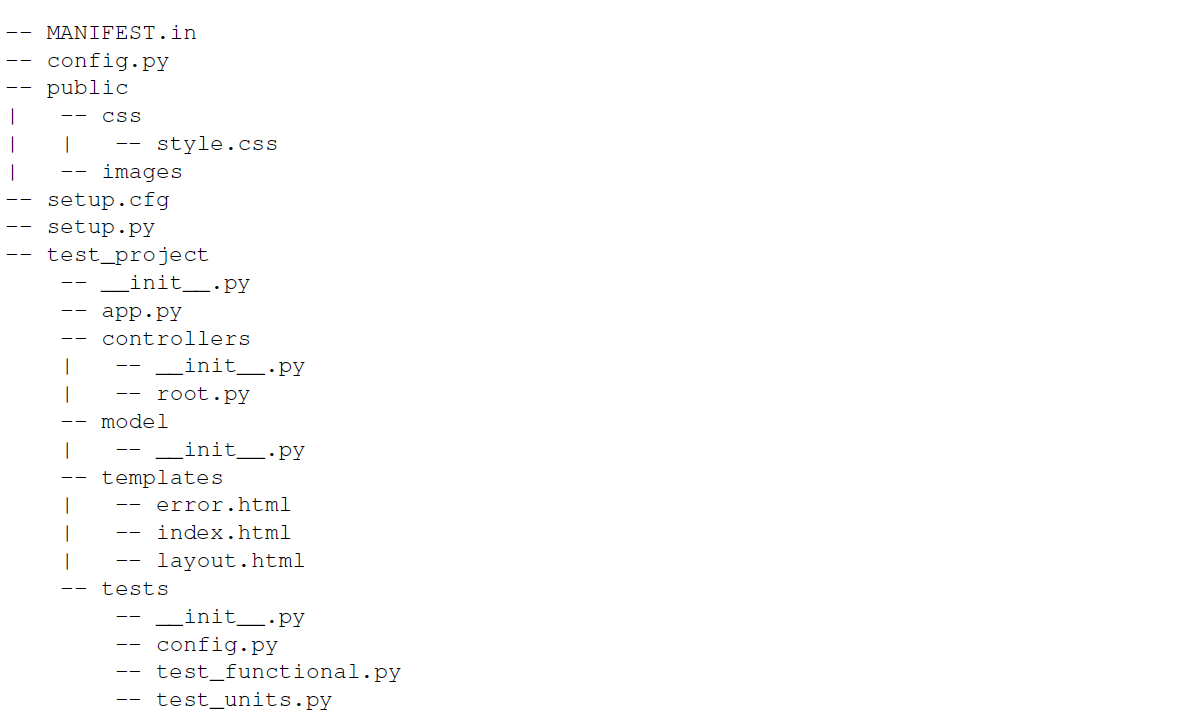
\includegraphics[width=\linewidth]{pecan.png}
  \caption{项目文件结构图}
  \label{fig:pecan}
\end{figure}

需要关注的主要有以下的文件:
\begin{itemize}
  \item config.py:提供Pecan项目的配置选项
  \item app.py:设定wsgi的app应用,以及其他的hook设定
  \item root.py:app所对应的路由处理模块,负责真正的业务处理
\end{itemize}

先从config.py文件开始看。文件的内容大致如下:
\begin{code-block}{python}
server = {
    'port': '8080',
    'host': '0.0.0.0'
}

# Pecan Application Configurations
app = {
    'root': 'test_project.controllers.root.RootController',
    'modules': ['test_project'],
    'static_root': '%(confdir)s/public',
    'template_path': '%(confdir)s/test_project/templates',
    'debug': True,
    'errors': {
        404: '/error/404',
        '__force_dict__': True
    }
}

logging = {
    'root': {'level': 'INFO', 'handlers': ['console']},
    'loggers': {
        'test_project': {'level': 'DEBUG', 'handlers': ['console']},
        'pecan': {'level': 'DEBUG', 'handlers': ['console']},
        'py.warnings': {'handlers': ['console']},
        '__force_dict__': True
    },
}
\end{code-block}

Server字典指定pecan项目的监听参数,port表示监听的端口,host表示监听地址。Logging
设定pecan的日志系统。App则是Pecan项目的核心,modules参数表示加载的模块,root表示
wsgi的app,其中注意的是,root指定的是app的入口类,而这个入口类需要包含在modules
当中。

分析app.py,其内容大致如下:
\begin{code-block}{python}
from pecan import make_app
from test_project import model


def setup_app(config):

    model.init_model()
    app_conf = dict(config.app)

    return make_app(
        app_conf.pop('root'),
        logging=getattr(config, 'logging', {}),
        **app_conf
    )
\end{code-block}

需要注意的就是make\_app,所有的app的初始化,都是有这个方法完成的,而make\_app有几个
重要的参数,一个是root,表示整个工程的app,一个是hooks,表示的是app的hook处理,而
另外一个则是wrap\_app,表示wsgi框架当中的中间件。该方法返回的是一个标准的wsgi的
app对象。因此,我们可以在其他的框架当中使用这个app对象,比如wsgiref,比如eventlet。

最后则是root.py文件,这是Pecan项目的实际处理模块。
\begin{code-block}{python}
from pecan import expose, redirect
from webob.exc import status_map


class RootController(object):

    @expose(generic=True, template='index.html')
    def index(self):
        return dict()

    @index.when(method='POST')
    def index_post(self, q):
        redirect('http://pecan.readthedocs.org/en/latest/search.html?q=%s' % q)

    @expose('error.html')
    def error(self, status):
        try:
            status = int(status)
        except ValueError:  # pragma: no cover
            status = 500
        message = getattr(status_map.get(status), 'explanation', '')
        return dict(status=status, message=message)
\end{code-block}

在以上的代码当中,需要注意的是expose这个方法。如果需要暴露api给外部访问,则对应的
方法上,就一定要添加expose注解器。关于expose的具体使用,请查看pydoc。
\begin{code-block}{python}
pecan.expose = expose(template=None, generic=False, route=None, **kw)
    Decorator used to flag controller methods as being "exposed" for
    access via HTTP, and to configure that access.

    :param template: The path to a template, relative to the base template
                     directory.
    :param content_type: The content-type to use for this template.
    :param generic: A boolean which flags this as a "generic" controller,
                    which uses generic functions based upon
                    ``functools.singledispatch`` generic functions.  Allows you
                    to split a single controller into multiple paths based upon
                    HTTP method.
    :param route: The name of the path segment to match (excluding
                  separator characters, like `/`).  Defaults to the name of
                  the function itself, but this can be used to resolve paths
                  which are not valid Python function names, e.g., if you
                  wanted to route a function to 'some-special-path'.
\end{code-block}

项目建立好之后,启动pecan项目,向外发布服务。
\begin{code-block}{bash}
pecan serve config.py
Starting server in PID 5901
serving on 0.0.0.0:8080, view at http://127.0.0.1:8080
\end{code-block}

使用浏览器访问发布的服务,如图 \colorunderlineref{fig:quickstart}所示
\begin{figure}[H]
  \centering
  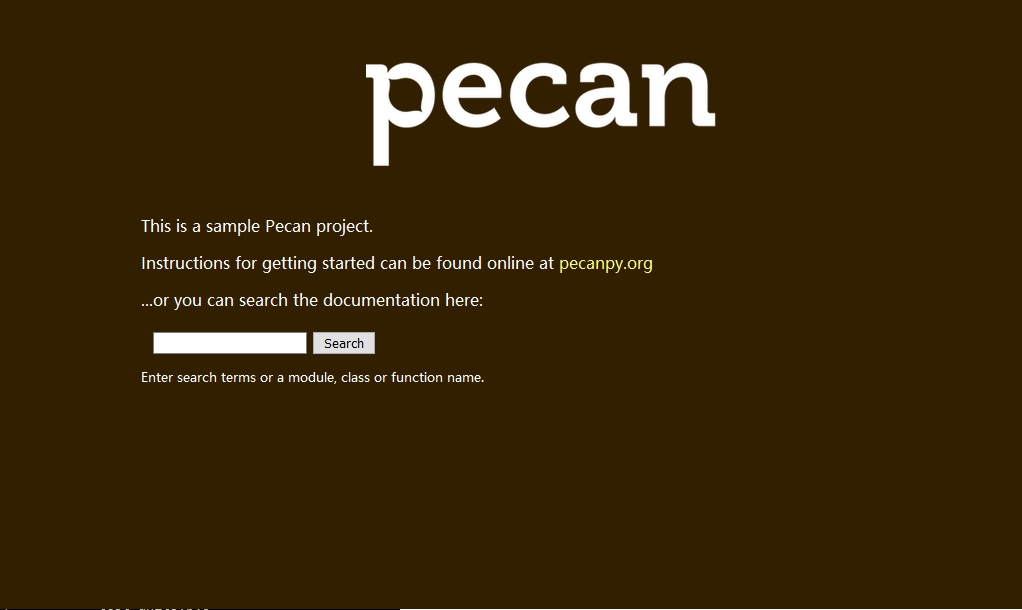
\includegraphics[width=\linewidth]{quickstart.png}
  \caption{返回结果}
  \label{fig:quickstart}
\end{figure}

\section{开发进阶}
在OpenStack Ironic,Vitrage,Neutron等项目中,Pecan被广泛的使用,但是,这些项目当中的Controller
却并不像上一节所看到的代码那样,而是使用的另外一种方式。这就是Pecan的另一种Controller
:RestController。
\begin{code-block}{python}
from pecan import expose
from pecan import rest
from pecan import response
import six
from six.moves import http_client
from webob import exc


class NodeController(rest.RestController):

    nic = NodeNicController()
    _custom_actions = {
        'start': ['POST'],
        'power-off': ['POST']
    }

    @expose(template='json')
    def get_all(self):
        return {'result': 'Call the method named get_all'}

    @expose(template='json')
    def get(self, nodeid):
        return {'result': 'Call the method named get', 'id': nodeid}

    @expose(template='json')
    def post(self, **body):
        response.status = http_client.ACCEPTED
        return {'node': body, 'method': 'post'}

    @expose(template='json')
    def put(self, nodeid, **body):
        response.status = http_client.ACCEPTED
        return {'body': body, 'id': nodeid}

    @expose(template='json')
    def delete(self, nodeid):
        response.status = http_client.NO_CONTENT
        return {'result': 'Call the method named delete', 'id': nodeid}

    @expose(template='json')
    def start(self, nodeid):
        response.status = http_client.ACCEPTED
        return {'result': 'Call the method named start', 'id': nodeid}

    def power_off(self, nodeid):
        response.status = http_client.ACCEPTED
        return {'result': 'Call the method named power_off', 'id': nodeid}


setattr(NodeController, 'power-off',
        expose(template='json')(
            six.get_method_function(NodeController.power_off)))


class VersionController(rest.RestController):

    @expose(template='json')
    def _default(self):
        return {'Version': 'v1.0'}


class RootController(rest.RestController):
    node = NodeController()
    version = VersionController()

    @expose()
    def _route(self, args, request):
        if request.content_type != 'application/json':
            raise exc.HTTPBadRequest('Not support content-type')
        return super(RootController, self)._route(args, request)
\end{code-block}

在这个例子当中,我们将详细讲述一下的几个内容:
\begin{itemize}
  \item 默认路由
  \item 构建路由
  \item 嵌套路由
  \item 请求预处理
  \item 默认处理
\end{itemize}

与\colorunderlineref{chap:start}章节不一样的是,在使用RestController的时候,Pecan提供了默认的路由信息。具体的
路由对照如下表
\begin{center}
  \rowcolors{2}{green!80!yellow!50}{green!70!yellow!40}
  \begin{tabularx}{\textwidth}{|X|X|X|}
  \hline
  Method & Description & URL \\ \hline
  get & Display one record & GET /nodes/1 \\
  get\_all & Display all records & GET /nodes \\
  post & Create a new record & POST /nodes \\
  put & Update an existing record & PUT /nodes/1 \\
  delete & Delete an existing record & DELETE /nodes/1 \\ \hline
  \end{tabularx}
  \label{tab:Pecan_URL_Mapping}
\end{center}

但很显然的是,以上的路由映射,并不能完全满足生产环境的需要。因此,Pecan提供了自定义
路由的机制。
\begin{code-block}{python}
class NodeController(rest.RestController):
    _custom_actions = {
        'start': ['POST'],
    }

    @expose(template='json')
    def start(self, nodeid):
        response.status = http_client.ACCEPTED
        return {'result': 'Call the method named start', 'id': nodeid}
\end{code-block}

在RestController当中,我们可以使用\_custom\_actions来实现自定义的路由信息。上述
代码自定义了一个start方法,则会新生成一个路由信息:当使用POST方法访问
/nodes/{node\_id}/start时,Pecan将会把请求转发到start方法。

在实际的环境中,我们还会遇到这样的url:\url{/os-host/{host-id}/power-off}。
如果按照上述所讲的,添加\_custom\_actions,可能会是这个样子

\begin{code-block}{python}
class NodeController(rest.RestController):
    _custom_actions = {
        'power-off': ['POST'],
    }

    @expose(template='json')
    def power-off(self, nodeid):
        ...
\end{code-block}

但这个明显是错误的,方法power-off不是一个合法的python命名。但是,如果我们将方法
power-off修改为power\_off,则又会出现404错误。这种情况该如何解决?
\begin{code-block}{python}
class NodeController(rest.RestController):

    _custom_actions = {
        'power-off': ['POST']
    }
    def power_off(self, nodeid):
        response.status = http_client.ACCEPTED
        return {'result': 'Call the method named power_off', 'id': nodeid}


setattr(NodeController, 'power-off',
        expose(template='json')(
            six.get_method_function(NodeController.power_off)))
\end{code-block}

到目前为止,我们解决了\url{/nodes}以及\url{/nodes/{node_id}/power-off}这类型的url的
处理,但是,如何解决接下来的url:\url{/nodes/{node_id}/nic/{nic_id}}?很显然,
这种属于嵌套的url,这就是我们接下来需要解决的问题。

\begin{code-block}{python}
class NodeController(rest.RestController):

    nic = NodeNicController()


class RootController(rest.RestController):

    node = NodeController()
    version = VersionController()
\end{code-block}

通过上述的代码,我们就神奇的构建了如下的url
\begin{code-block}{python}
/version
/node
/node/{node_id}/nic
/node/{node_id}/nic/{nic_id}
\end{code-block}

在以上的代码中,我们简介了如何使用pecan。但是,关于真正的参数处理,以及其他的一些问题,我们还没有解决。

\section{强大的参数校验}
依然从代码中讲解
\begin{code-block}{python}
from datetime import datetime
import pecan
from pecan import expose
from pecan import rest
import six
from six.moves import http_client
import uuid
from webob import exc
import wsme
from wsmeext.pecan import wsexpose
from wsme import types as wtypes


class Node(wtypes.Base):

    name = wsme.wsattr(wtypes.text, mandatory=True)
    uuid = wsme.wsattr(datatypes.uuidtype, readonly=True)
    console_enabled = datatypes.booleantype
    power_state = wsme.wsattr(
        wtypes.Enum(str, 'power-on', 'power-off'), mandatory=True)
    raid_config = wsme.wsattr({wtypes.text: datatypes.jsontype})
    disks = [wtypes.text]
    update_time = datetime

    _classis_uuid = None

    def _get_classis_uuid(self):
        return self._classis_uuid

    def _set_classis_uuid(self, value):
        if value:
            self._classis_uuid = value
        elif value == wtypes.Unset:
            self._classis_uuid = wtypes.Unset

    classis_uuid = wsme.wsproperty(datatypes.uuidtype, _get_classis_uuid,
                                   _set_classis_uuid)


class NodeController(rest.RestController):

    _custom_actions = {
        'power-operate': ['POST'],
        'start': ['GET']
    }

    @wsexpose(Node, datatypes.uuidtype, wtypes.text,
              datatypes.uuidtype, int, int, bool)
    def get(self, nodeid, name=None, uuid=None,
            page=None, limit=None, show_all=False):
        node = Node()
        node.name = 'node1'
        node.console_enabled = True
        node.power_state = 'power-on'
        node.raid_config = dict(name='lucifer')
        node.disks = ['/dev/sda', '/dev/sdb']
        return node
\end{code-block}

在上述代码中,我们的NodeController不再使用expose注解器,而是使用wsexpose注解器。
Wsexpose接受多个参数。第一个参数为方法的返回类型,倒数第二个参数为request的body类型,
最后一个参数为response的返回状态码,其余参数,表示的是传递的参数的类型。使用该注解器
的意图是,所有的入参,返回值,request的body以及response的状态码,都在注解器中进行校验
和处理。

Node为一个自定义的返回数据类型。该数据类型由name,uuid等等数据元素组成。Name的数据类型
为字符串类型,mandatory表示是必须;readonly表示作为入参时,uuid是不允许设置的;Enum表示
数据类型为枚举类型,这些枚举类型的数据元素类型为str,可选的值为power-on和power-off;
wsme.wsattr({})表示参数的类型为一个字典;同样的,[]表示参数的类型为列表。
